\documentclass[11pt]{article}
\usepackage[utf8]{inputenc}
\usepackage[T1]{fontenc}
\usepackage[brazilian]{babel}
\usepackage{graphicx}
\usepackage{longtable}
\usepackage{wrapfig}
\usepackage{rotating}
\usepackage[normalem]{ulem}
\usepackage{amsmath}
\usepackage{amssymb}
\usepackage{capt-of}
\usepackage{hyperref}
\usepackage{geometry}
\usepackage{booktabs}
\usepackage{url}
\usepackage{hyperref}
\usepackage{multicol}
\usepackage{algorithm}
\usepackage{algorithmicx}
\usepackage[noend]{algpseudocode}
\usepackage[title]{appendix}
\usepackage{float}

% \bibliographystyle{unsrtnat}

\geometry{a4paper, left=20mm, top=35mm, bottom=35mm, right=20mm}

\author{
    Adolfo Aires Schneider (234991) \\
    Ieremies Romero (217938) \\
    Lucas Guesser Targino da Silva (203534)}
\date{\today}
\title{MO824 - Algoritmos Genéticos}

\begin{document}

\maketitle
\section{Descrição do problema}
\label{sec:descricao}
No problema \emph{Maximum Quadratic Binary Function} (MAX-QBF), proposto em \cite{bib:qbf-survey},  temos que maximizar a função \(f: \mathbb{B}^{|x|} \to \mathbb{R}\), onde \(|x|\) é a dimensão do problema, descrita como:

\begin{alignat*}{6}
    max & \quad && \displaystyle{\sum_{i = 1} ^n \sum_{j = 1} ^n a_{ij} x_i x_j}&\\
    &&& x_i \in \{0, 1\}& \text{para todo i }\in \{1,..,n\},
\end{alignat*}

\noindent em que \(a_{i,j} \in \mathbb{R} \ (i,j = 1,\dots,n)\) são os coeficientes da função, dados como parâmetros do problema.

A este problema adicionamos a restrição
\[ \sum_{i=1}^{n} w_{i} x_{i} \leq W ,\]
onde \(w_{i}\) é dito o peso da variável $x_{i}$. Nessa nova versão chamada \textit{Maximum Knapsack quadratic binary function}~(MAX-KQBF), continuamos tendo por objetivo maximizar a função $f$, mas desta vez também precisamos satisfazer a restrição que a soma dos pesos das variáveis na solução não exceda \(W\). Veja que podemos ver esse problema como um conjunto de itens $x$, onde cada item $i \in x$ tem um peso $w_i$, nos quais devem ser empacotados em uma mochila de capacidade W. Neste caso, as variáveis de decisão $x_i$, consiste em escolher se o item $i$ está ou não na mochila (que representa a solução), onde $x_i = 1$ se o item $i$ estiver na solução.

Durante esse relatório, nos referiremos a $\delta (x_{i})$ como o custo que o elemento $x_{i}$ incumbe a atual solução $X$. Caso $x_{i}$ não esteja na solução $X$, então $\delta (x_i) = f(X \cup \{x_i\}) - f(X)$. Caso $x_{i}$ já esteja na solução $X$, então $\delta (x_i) = f(X \setminus \{x_i\}) - f(X)$.

\section{Metodologia}
\label{sec:metodologia}
Nessa atividade, utilizaremos \textbf{Algoritmos Genéticos} (GA) como nossa meta-heurística.
\section{Codificação de uma solução}
\label{sec:org3138bfb}

Uma característica interessante de GA é sua separação da representação e suas variáveis. Tomando como inspiração a biologia, o \textbf{genótipo} de é uma representação codificada das variáveis. Assim, o vetor \(x\) é representado por uma string \(s\) de tamanho \(l\) feita de símbolos no alfabeto \(A\) usando o mapeamento \(c\).

O comprimento da string depende tanto do tamanho do alfabeto como do tamanho do espaço de busca do problema. Cada elemento da string é dito \textbf{gene} e seus possíveis valores são chamadas \textbf{alelos}.

Assim, na prática, precisamos encontrar
\[ \arg\, \min \limits_{s \in A^{l}} g(s) \]
tal que \(g(s) = f(c(s))\), onde \(f\) é a função a ser minimizada no espaço de busca original.

Dessa forma, tomando como inspiração o comportamento de seleção natural, os descendentes de uma população (conjunto de soluções) devem ter as características mais "desejáveis". Estas, são determinadas por favorecer aqueles cromossomos (strings acima referenciadas) com maior aptidão, uma função real de \(f\), monotônica, não negativa. A estratégia de escolha de tal função tem por objetivo favorecer aqueles cromossomos que fornecem as melhores soluções para o problema original.

Tais descendentes, acima mencionados, são gerados a partir do cruzamento de cromossomos e mutação. Para o operador de cruzamento (\emph{crossover}), é comum utilizarmos a troca de um ou mais alelos entre os parentes. Já para a mutação, é escolhido um conjunto de alelos randomicamente para terem seus valores alterados.

Podemos repetir esse processo e, a cada iteração, produzir uma nova geração de cromossomos até que estejamos satisfeitos. Um algoritmo de alto nível, retirado de \cite{bib:genetic-algorithm}, é apresentado no Algoritmo \ref{algo:ga}.

\begin{algorithm}
    \caption{Genetic-Algorithm}
    \label{algo:ga}
    \begin{algorithmic}[1]
        \State{escolher a população inicial de cromossomos}
        \While{condição de parada não é satisfeita}
            \While{Não há descendentes suficientes}
                \If{condição de cruzamento é satisfeita}
                    \State{Selecionar cromossomos pai}
                    \State{Selecionar parâmetros de cruzamento}
                    \State{Executar cruzamento}
                \EndIf
                \If{condição de mutação é satisfeita}
                    \State{Selecionar pontos de mutação}
                    \State{Executar mutação}
                \EndIf
                \State{Calcular adaptação (fitness) dos descendentes}
            \EndWhile
            \State{Selecionar nova população}
        \EndWhile
        \State{\textbf{return} Melhor cromossomo da população}
    \end{algorithmic}
\end{algorithm}

\section{População inicial}
\label{sec:org7eb563e}
É possível perceber que o tamanho da população utilizada irá diretamente influenciar a qualidade das soluções e o tempo de execução. Populações grandes significam uma busca mais ampla e, possivelmente, melhores soluções ao custo de um tempo maior de execução. Assim, precisa-se encontrar um balanço.

Como proposto em \cite{bib:genetic-algorithm}, podemos utilizar a ideia de que todo o espaço de busca deve ser acessível pelo \emph{crossover} da população inicial. Para tal, cada valor do nosso alfabeto (alelo) deve aparecer em cada posição da ‘string’ (‘locus’).

Uma vez determinado o tamanho, é necessário ainda escolher a população inicial. De forma geral, a literatura aponta que uma simples amostragem sem repetição é suficiente, mas formas mais refinadas já foram propostas com objetivo de garantir a cobertura do espaço de busca, mencionado acima. Além disso, podemos ``semear'' a população inicial com boas soluções já obtidas por outros métodos.

\section{Seleção e Reprodução}
\label{sec:org9a82437}
Para produzirmos a próxima geração, precisamos selecionar aqueles indivíduos que serão ``reproduzidos''. Fazemos isso pelo método estilo \textbf{torneio}, onde dois cromossomos são escolhidos aleatoriamente e o melhor dos dois (em relação à função de aptidão) é escolhido para continuar enquanto o outro é descartado. Assim, nossas populações entre gerações mantém os melhores indivíduos em comum, enquanto inserimos novos para ampliar a busca.

Visto que a população conterá duplicatas, precisamos reconstruí-la utilizando o \emph{crossover}. No nosso caso, utilizamos \textbf{\emph{two point crossover}} (\texttt{2X}) como o método de produzir novas soluções. Para dois cromossomos, ditos pais, construímos dois descendentes. Cada um é a cópia de um dos pais com um intervalo do locus do outro pai, conforme exemplificado na Figura \ref{fig:crossover}. As duas posições, em vermelho na figura, são escolhidas aleatoriamente.

É importante, nesse ponto, ressaltar que nem todo cromossomo gerado corresponde a uma solução viável ao problema original. Porém, estes serão descartados já que a nossa função de aptidão retorna menos infinito para soluções inviáveis ao problema.

\begin{figure}
    \centering
    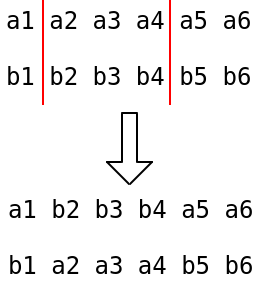
\includegraphics[width=0.2\textwidth]{figures/two_points_crossover.png}
    \caption{Representação esquemática do \textbf{\emph{two point crossover}} (\texttt{2X}).}
    \label{fig:crossover}
\end{figure}

\section{Mutação}

Como discutido anteriormente, é importante que haja uma taxa de mutação a cada reprodução para ser mantida a diversidade da população. Implementamo-na a partir da \textbf{taxa de mutação} \(M\) que representa a chance de cada alelo em cada descendente de uma geração sofrer uma mutação. Caso isso ocorra, o valor dele é alterado. Iremos experimentar com diferentes valores para esta taxa.

\section{Critério de parada}

Critérios de parada mais simples, e também mais comuns na literatura, são:

\begin{enumerate}
    \item limitar o tempo de execução;
    \item limitar o número de gerações geradas;
\end{enumerate} 

Porém, critérios que consideram os resultados obtidos pelo algoritmo também podem ser utilizados:

\begin{enumerate}
    \item parar quando a diversidade da população é baixa;
    \item parar quando a solução não melhora após algumas gerações;
\end{enumerate}

\section{Estratégias evolutivas alternativas}
\label{sec:alternativas}

As estratégias evolutivas alternativas utilizadas no desenvolvimento foram \textit{Steady-State $\lambda +	\mu$} e \textit{Manutenção de diversidade}, ambas são descritas abaixo.

\subsection{Steady-State $\lambda +	\mu$}
Uma das estratégias alternativas implementadas é uma variante da estratégia \textit{Steady-State}, a estratégia $\lambda +	\mu$. Nessa variante, em cada iteração, $\mu$ \textit{offsprings} são gerados, os melhores  $\lambda$  indivíduos do conjunto união dos \textit{parents} e \textit{offsprings} são escolhidos para compor a nova população. Na implementação feita tanto $\lambda$ quanto $\mu$ foram definidos como o tamanho da população. O objetivo dessa abordagem consiste em não perder soluções consideradas boas de uma geração para a próxima, porém podendo levar o algoritmo apresentar uma convergência prematura e uma baixa diversidade. Para balancear esse fator, a próxima estratégia evolutiva alternativa utilizada procura aumentar a diversidade do algoritmo genético.

\subsection{\textit{Manutenção de diversidade}}
\label{sec:diversidade}

A diversidade da população é um fator importante para um algoritmo genético conseguir explorar de forma ampla o espaço de soluções. Diversos métodos podem ser aplicados com objetivo de aumentar essa diversidade, como criar uma população de maneira mais uniforme, aumentar o tamanho da população ou taxa de mutação e também evitar gerar indivíduos repetidos entre gerações. Para essa última abordagem existe a estratégia alternativa chamada de Manutenção de Diversidade, cujo possui o objetivo de evitar que os \textit{offsprings} sejam meras duplicatas dos indivíduos que as formaram. 

Para evitar duplicatas, uma forma seria a comparação dos indivíduos com os novos candidatos, adicionando um esforço computacional maior e mais perceptível em grandes populações. A estratégia utilizada limita os possíveis \textit{crossover-points} no intervalo $[L, R]$ com $L$ e $R \in \{1, ..., n\}$ e $R >= L$ de uma forma a tentar diminuir a chance de ocorrerem duplicatas, onde \(L\) é o primeiro locus com alelo diferentes entre os pais e \(R\) o último. Assim, as chances do descendente gerado ser igual são reduzidas.

\section{Implementação}
\label{sec:implementacao}

Partimos de uma configuração padrão:

\begin{enumerate}
    \item Tamanho da população: $P_1 = 100$;
    \item Taxa de mutação: $M_1 = 1\%$;
    \item População inicial construída aleatoriamente\footnote{Criamos um cromossomo com todos os alelos desativados e ativamos alguns deles aleatoriamente, respeitando as restrições do problema em questão.}
    \item \textbf{\emph{two point crossover}} (\texttt{2X});
    \item Critério de parada: 1000 gerações;
\end{enumerate}

Estudamos \(5\) configurações, alterando apenas um aspecto por vez\footnote{Quando não explicitado, os parâmetros se mantém igual à configuração padrão.}:

\begin{description}
\item[{Configuração \(1\)}] PADRÂO: Algoritmo genético com tamanho de população $P_1$, taxa de mutação $M_1$ e construção aleatória da população.
\item[{Configuração \(2\)}] PADRÃO + POP: Algoritmo genético PADRÃO, mas com tamanho de população $P_2$.
\item[{Configuração \(3\)}] PADRÃO + MUT: Algoritmo genético PADRÃO, mas com taxa de mutação $M_2$.
\item[{Configuração \(4\)}] PADRÃO + EVOL1: Algoritmo genético PADRÃO, mas com estratégia evolutiva alternativa 1 (X).
\item[{Configuração \(5\)}] PADRÃO + EVOL2: Algoritmo genético PADRÃO, mas com estratégia evolutiva alternativa 2 (X).
\end{description}

Selecionamos para os experimentos $P_2 = 300$ e $M_2 = 0.5\%$.

\section{Análise dos resultados}
\label{sec:analysis}

\subsection{Taxa de mutação}

Comparando as Tabelas \ref{table:result-vanilla} e \ref{table:result-vanilla-mutation-05-percent}, observamos que uma taxa de mutação menor levou a resultados um pouco melhores. Na verdade, a diferença é mais evidente em instâncias maiores, como a 200 e 400, já que em instâncias menores ambos chegaram ao mesmo resultado. A mutação, de certa forma, representa uma busca local, no sentido que são feitas modificações nas soluções conhecidas a fim de explorar a vizinhança. Assim, taxas de mutações maiores estão relacionadas a maior diversificação, enquanto que taxas menores estão relacionadas a intensificação. Assim, faz-se necessário escolher um valor para a taxa de mutação que consiga dosar os dois corretamente.

Por causa da forma com que foi implementada, esse balanço entre intensificação e diversificação controlado pela taxa de mutação é influenciado pelo número de genes de um cromossomo: cromossomos maiores sofrem, estatisticamente, mais modificações do que cromossomos menores.

Voltando para a comparação dos resultados, vemos que para instâncias grandes, a taxa de mutação está muito alta, não permitindo o algoritmo acumular características boas de uma solução para a outra. Por isso, seria interessante em trabalhos futuros investigar uma taxa de mutação adaptativa, que considerasse o número de genes de um cromossomo.

\subsection{Tamanho da população}

Comparando as Tabelas \ref{table:result-vanilla} e \ref{table:result-vanilla-population-300} observamos melhores resultados em geral ao custo de um aumento proporcional no tempo computacional (aproximadamente três vezes maior em cada instância).

A melhora da solução obtida pode ser explicada pelo fato do algoritmo explorar mais o domínio de solução.

Em alguns casos houve piora da solução entretanto. Populações maiores reduzem as chances de indivíduos bons se reproduzirem, e caso a diversidade da população estiver alta, isso pode ser um problema. Nesses casos, utilizar soluções como a estratégia evolutiva alternativa $\lambda + \mu$ seja uma boa alternativa.

\subsection{\textit{Manutenção de diversidade}}

Comparando as Tabelas \ref{table:result-vanilla} e \ref{table:result-diversification-maintenance} observamos que praticamente não houve modificação nos resultados. A estratégia evolutiva alternativa \textit{Manutenção de diversidade} mostrou-se equivalente à proposta original.

Uma explicação para tal resultado pode estar na similaridade entre as duas. Apesar de haver diferença em como os pontos de cruzamento são selecionados, em ambos eles ainda são bastante similares.


\subsection{Steady-State $\lambda +	\mu$}

Comparando as Tabelas \ref{table:result-vanilla} e \ref{table:result-steady}, observamos melhora dos resultados, principalmente nas instâncias maiores.

O algoritmo genético é baseado e gerar descendentes que combinam características boas dos pais. Isso significa que quanto melhores forem as características dos pais, melhores serão as dos filhos. A estratégia original propõe a próxima geração ser todos os filhos (exceto o prior deles) mais a melhor solução até então encontrada. Mas nem todos os filhos têm características boas. Pode ser que alguns filhos combinem apenas as características ruins dos pais. Dessa forma, é interessante considerar manter os pais ao invés dos filhos quando for vantajoso, que é justamente o que a estratégia Steady-State $\lambda +	\mu$ faz.

Por outro lado, observamos um aumento consideravel no tempo computacional. Isso pode ser explicado pela operação necessária para selecionar os melhores elementos entre os pais e filhos, que envolve uma operação de ordenação.

\bibliographystyle{ieeetr}
\bibliography{bibliography}

\begin{appendices}

\section{Implementação e execução dos experimentos}

O problema foi executado num ideapad S145 81S90005BR: Lenovo IdeaPad S145 Notebook Intel Core i5-8265U (6MB Cache, 1.6GHz, 8 cores), 8GB DDR4-SDRAM, 460 GB SSD, Intel UHD Graphics 620.

O sistema operacional foi o Fedora 35 executando o Java 17 e Gradle 7.4.

O desenvolvimento da solução do problema foi feito em Java, baseado no framework disponibilizado pelo professor, e o código pode ser encontrado em \cite{bib:github}.

\section{Instâncias}

As instâncias utilizadas nos experimentos foram disponibilizadas pelo professor da disciplina e diferem essencialmente na quantidade de variáveis $|x|$, havendo uma progressão no tamanho da mochila $W$ com o aumento de $|x|$.

\section{Resultado dos experimentos computacionais}

\begin{itemize}
    \item \textit{n. gen}: número de gerações, utilizado como critério de parada;
    \item \textit{mut rate}: taxa de mutação;
    \item \textit{pop size}: tamanho da população;
    \item \textit{k. capac.}: capacidade da mochila;
    \item \textit{sol. w}: peso da solução, para verificarmos que a restrição de limite de peso é satisfeita;
    \item \textit{exec t.}: tempo de execução em segundos;
    \item \textit{sol. cost}: valor da função objetivo (custo da solução encontrada);
\end{itemize}

\begin{table}[H]
\centering
\begin{tabular}{lrrrrrrrr}
\toprule
{} &  instances &  n. gen &  mut rate &  pop size &  k. capac. &  sol. w &  exec t. [s] &  sol. cost \\
\midrule
0 &         20 &    1000 &      0.01 &       100 &         64 &      54 &        0.918 &        120 \\
1 &         40 &    1000 &      0.01 &       100 &        138 &     132 &        2.648 &        303 \\
2 &         60 &    1000 &      0.01 &       100 &        221 &     221 &        5.082 &        470 \\
3 &         80 &    1000 &      0.01 &       100 &        288 &     286 &        9.090 &        733 \\
4 &        100 &    1000 &      0.01 &       100 &        346 &     345 &       13.646 &       1249 \\
5 &        200 &    1000 &      0.01 &       100 &        680 &     671 &       54.607 &       3613 \\
6 &        400 &    1000 &      0.01 &       100 &       1344 &    1338 &      221.373 &       7884 \\
\bottomrule
\end{tabular}
\caption{Solução obtida com o algoritmo genético não modificado para cada configuração e instância do problema.}
\label{table:result-vanilla}
\end{table}
\begin{table}[H]
\centering
\begin{tabular}{lrrrrrrrr}
\toprule
{} &  instances &  n. gen &  mut rate &  pop size &  k. capac. &  sol. w &  exec t. [s] &  sol. cost \\
\midrule
0 &         20 &    1000 &     0.005 &       100 &         64 &      54 &        0.974 &        120 \\
1 &         40 &    1000 &     0.005 &       100 &        138 &     132 &        3.200 &        303 \\
2 &         60 &    1000 &     0.005 &       100 &        221 &     217 &        5.529 &        481 \\
3 &         80 &    1000 &     0.005 &       100 &        288 &     288 &        9.627 &        766 \\
4 &        100 &    1000 &     0.005 &       100 &        346 &     345 &       15.386 &       1237 \\
5 &        200 &    1000 &     0.005 &       100 &        680 &     678 &       62.351 &       3714 \\
6 &        400 &    1000 &     0.005 &       100 &       1344 &    1344 &      245.488 &       9200 \\
\bottomrule
\end{tabular}
\caption{Solução obtida com o algoritmo genético não modificado para cada configuração e instância do problema.}
\label{table:result-vanilla-mutation-05-percent}
\end{table}
\documentclass{article}
\usepackage[utf8]{inputenc}
\usepackage{booktabs}

\begin{document}

\begin{table}
\centering
\begin{tabular}{lrrrrrrrr}
\toprule
{} &  instances &  n. gen &  mut rate &  pop size &  k. capac. &  sol. w &  exec t. [s] &  sol. cost \\
\midrule
0 &         20 &    1000 &      0.01 &       300 &         64 &      54 &        2.411 &        120 \\
1 &         40 &    1000 &      0.01 &       300 &        138 &     133 &        7.634 &        307 \\
2 &         60 &    1000 &      0.01 &       300 &        221 &     212 &       16.005 &        491 \\
3 &         80 &    1000 &      0.01 &       300 &        288 &     282 &       27.461 &        783 \\
4 &        100 &    1000 &      0.01 &       300 &        346 &     346 &       41.520 &       1208 \\
5 &        200 &    1000 &      0.01 &       300 &        680 &     679 &      165.724 &       3550 \\
6 &        400 &    1000 &      0.01 &       300 &       1344 &    1339 &      723.375 &       8240 \\
\bottomrule
\end{tabular}
\caption{Solução obtida para cada configuração e instância do problema.}
\label{table:all-data}
\end{table}


\end{document}

\begin{table}[H]
\centering
\begin{tabular}{lrrrrrrrr}
\toprule
{} &  instances &  n. gen &  mut rate &  pop size &  k. capac. &  sol. w &  exec t. [s] &  sol. cost \\
\midrule
0 &         20 &    1000 &      0.01 &       100 &         64 &      56 &        3.015 &        120 \\
1 &         40 &    1000 &      0.01 &       100 &        138 &     136 &       10.860 &        305 \\
2 &         60 &    1000 &      0.01 &       100 &        221 &     217 &       23.954 &        453 \\
3 &         80 &    1000 &      0.01 &       100 &        288 &     288 &       46.665 &        781 \\
4 &        100 &    1000 &      0.01 &       100 &        346 &     346 &       76.459 &       1187 \\
5 &        200 &    1000 &      0.01 &       100 &        680 &     679 &      254.404 &       3889 \\
6 &        400 &    1000 &      0.01 &       100 &       1344 &    1344 &     1204.936 &      10227 \\
\bottomrule
\end{tabular}
\caption{Solução obtida com o algoritmo genético com estratégia adaptativa alternativa Steady-State $\lambda + \mu$ para cada configuração e instância do problema.}
\label{table:result-steady}
\end{table}
\documentclass{article}
\usepackage[utf8]{inputenc}
\usepackage{booktabs}

\begin{document}

\begin{table}
\centering
\begin{tabular}{lrrrrrrrr}
\toprule
{} &  instances &  n. gen &  mut rate &  pop size &  k. capac. &  sol. w &  exec t. [s] &  sol. cost \\
\midrule
0 &         20 &    1000 &      0.01 &       100 &         64 &      54 &        1.033 &        120 \\
1 &         40 &    1000 &      0.01 &       100 &        138 &     138 &        2.968 &        279 \\
2 &         60 &    1000 &      0.01 &       100 &        221 &     221 &        5.415 &        481 \\
3 &         80 &    1000 &      0.01 &       100 &        288 &     285 &        9.852 &        776 \\
4 &        100 &    1000 &      0.01 &       100 &        346 &     341 &       14.252 &       1166 \\
5 &        200 &    1000 &      0.01 &       100 &        680 &     679 &       59.862 &       3457 \\
6 &        400 &    1000 &      0.01 &       100 &       1344 &    1339 &      257.981 &       7717 \\
\bottomrule
\end{tabular}
\caption{Solução obtida para cada configuração e instância do problema.}
\label{table:all-data}
\end{table}


\end{document}


\section{Resultados esperados}

Abaixo está uma tabela que indica o intervalo no qual está a solução ótima para cada instância do problema.

\begin{table}[H]
    \centering
    \begin{tabular}{cc}
    % & \cline{1-2} \\
    $|x|$ & \multicolumn{1}{l}{MAX-KQBF} \\\hline
    $20$ & [80,151] \\
    $40$ & [275,429] \\
    $60$ & [446, 576] \\
    $80$ & [729,1000] \\
    $100$ & [851, 1539] \\
    $200$ & [3597, 5826] \\
    $400$ & [10846, 16625]
    \end{tabular}
    \caption{Tabela com os intervalos de resultado esperados para cada instância.}
    \label{table:intervalos}
\end{table}

\end{appendices}

\end{document}
